\documentclass[11pt]{article}

%% LaTeX Preamble - Common packages

\usepackage[utf8]{inputenc}
\usepackage[spanish]{babel}
\usepackage{graphicx}
\usepackage{amsmath,amssymb}
\usepackage[left=2cm,right=2cm,top=2cm,bottom=2cm]{geometry}

\spanishdecimal{.}

\title{Examen rápido No. 4}
\author{Reconocimiento de Patrones (2023-2)}
\date{Julio Waissman Vilanova} % delete this line to display the current date

%%% BEGIN DOCUMENT
\begin{document}

\maketitle

\vspace{5mm}

\textbf{Nombre}: \line(1,0){400}

\vspace{9mm}


\begin{enumerate}



\item Considera las siguientes figuras A y B

\begin{center}
  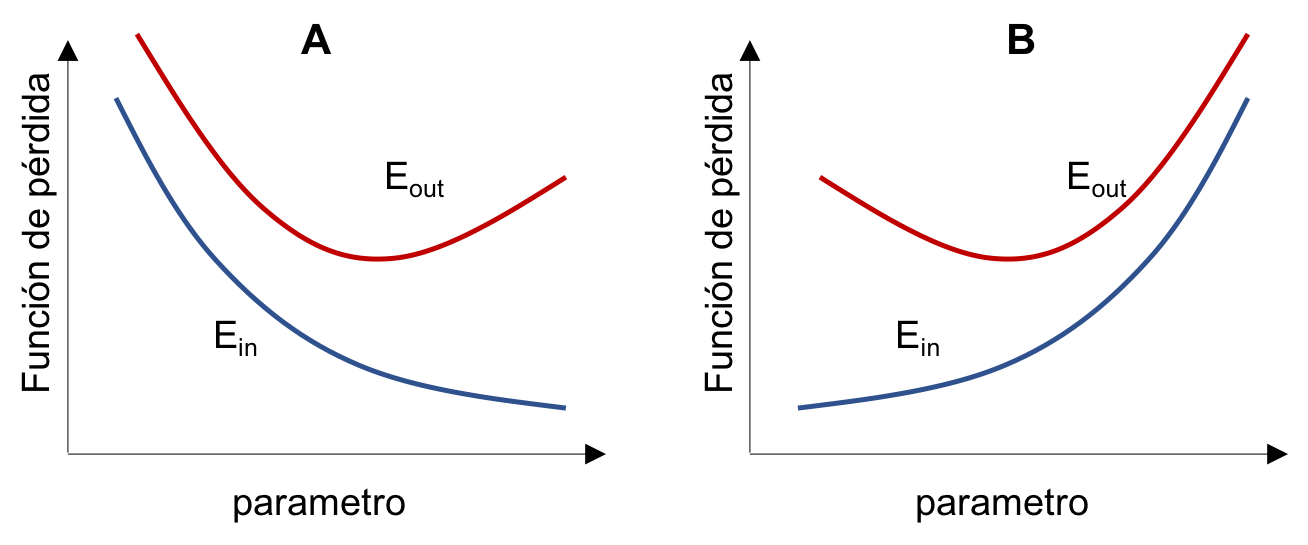
\includegraphics[width = 0.8\textwidth]{curvas.png}
\end{center}

Asigna cual es la curva sobre los errores en muestra $E_{in}$ y fuera de muestra
$E_{out}$ que debería salir teóricamente para los siguientes parámetros de
ajuste de métodos de aprendizaje:
\begin{itemize}
\item[ A B ] Número de neuronas en la capa oculta en una red neuronal.
\item[ A B ] Parámetro $\lambda$ de regularización en regresión lineal.
\item[ A B ] Umbral $\gamma$ entre 0 y 1 que es el valor por el cual se considera que un objeto pertenece a la clase 1 en regresión logística (por default $\gamma = 0.5$.
\item[ A B ] Valor de $C$ es una SVM con kernel lineal.
\item[ A B ] Número de capas ocultas en una red neuronal.
\item[ A B ] Parámetro $\sigma$ utilizado en el kernel gaussiano para una SVM.
\end{itemize}

\newpage


\item Supongamos que se esta resolviendo un problema de análisis de sentimientos
  en documentos utilizando como método para clasificar los diferentes
  sentimientos que se pueden obtener de un \emph{twit} utilizando un algoritmo
  basado en regresión logística. Si tenemos al rededor de 5000 palabras
  diferentes en nuestra \emph{bolsa de palabras}, 4 sentimientos básicos
  (<<satisfecho>>, <<molesto>>, <<triste>>, <<otro>>) y al rededor de 20,000
  \emph{twits} previamente clasificados.

  Si realizamos una curva de aprendizaje y obtenemos algo similar a la curva
  siguiente:

\begin{center}
  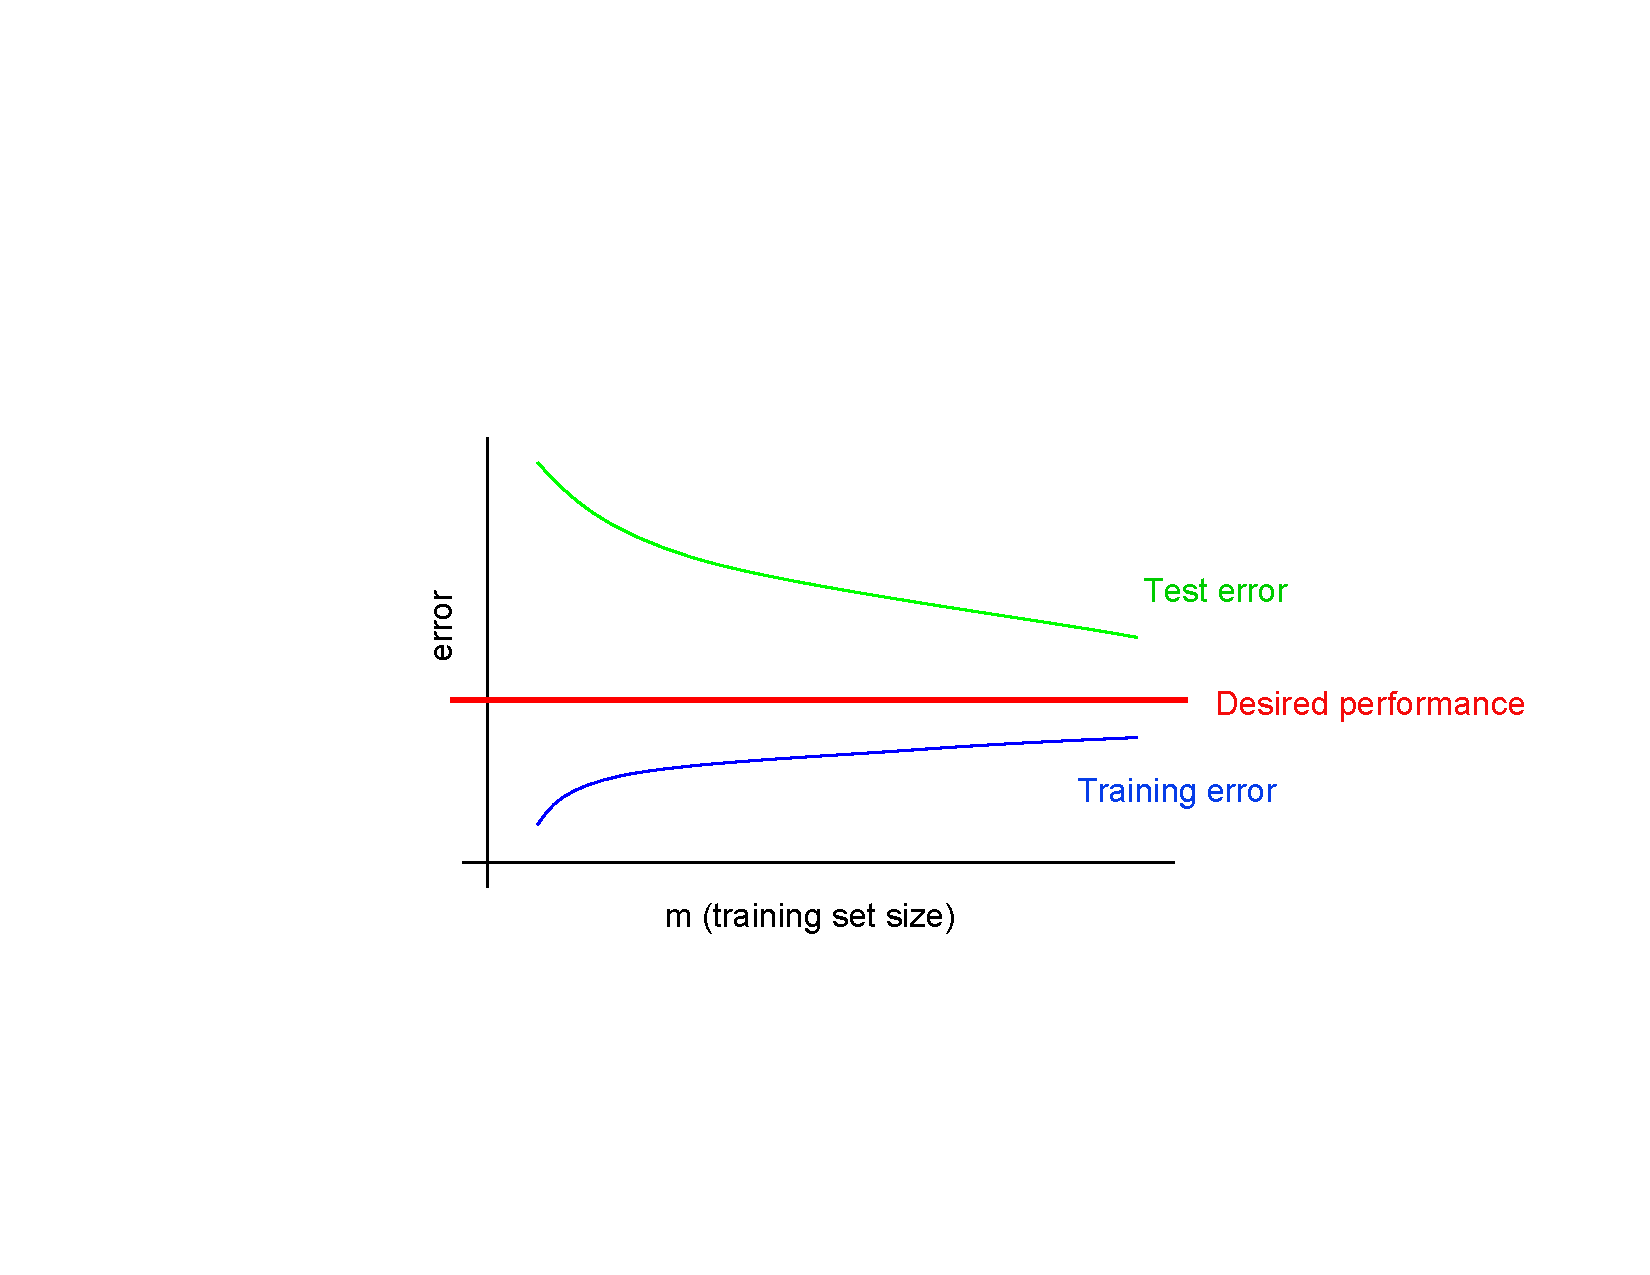
\includegraphics[width = 0.8\textwidth]{h_var.pdf}
\end{center}
subraya las acciones que podrían mejorar al sistema de aprendizaje.

\begin{itemize}
\item Tratar de generar más \emph{tuits} clasificados.
\item Tratar de reducir el número de palabras de la \emph{bolsa de palabras}.
\item Tratar de aumentar las palabras de la \emph{bolsa de palabras}.
\item Agregar otras características como la longitud del \emph{tuit} o la hora a
  la que fue enviado.
\item Aumentar el número máximo de iteraciones del algoritmo de optimización.
\item Aumentar el valor de $\lambda$ (parámetro de regularización).
\item Disminuir el valor de $\lambda$ (parámetro de regularización).
\item Utilizar una SVM con kernel gaussiano.
\end{itemize}

\item Supongamos que estamos estimando la demanda de energia eléctrica doméstica
  en la Cd. de Hermosillo para el próximo día, utilizando como información el
  consumo de energía eléctrica de los 30 días anteriores, la temperatura máxima
  en Hermosillo de los 30 días anteriores, la temperatura mínima en Hermosillo
  de los 30 días anteriores, el día de la semana, una variable que indica si el
  día es festivo o no y una variable que indica la estación del año (invierno,
  primavera, verano y otoño). Se aplica un método de regresión lineal con la
  información de los últimos 5 años.

  Para analizar el desempeño del algoritmo de regresión lineal, se realiza una
  curva de aprendizaje la cual resulta ser de la forma siguiente:

  \begin{center}
    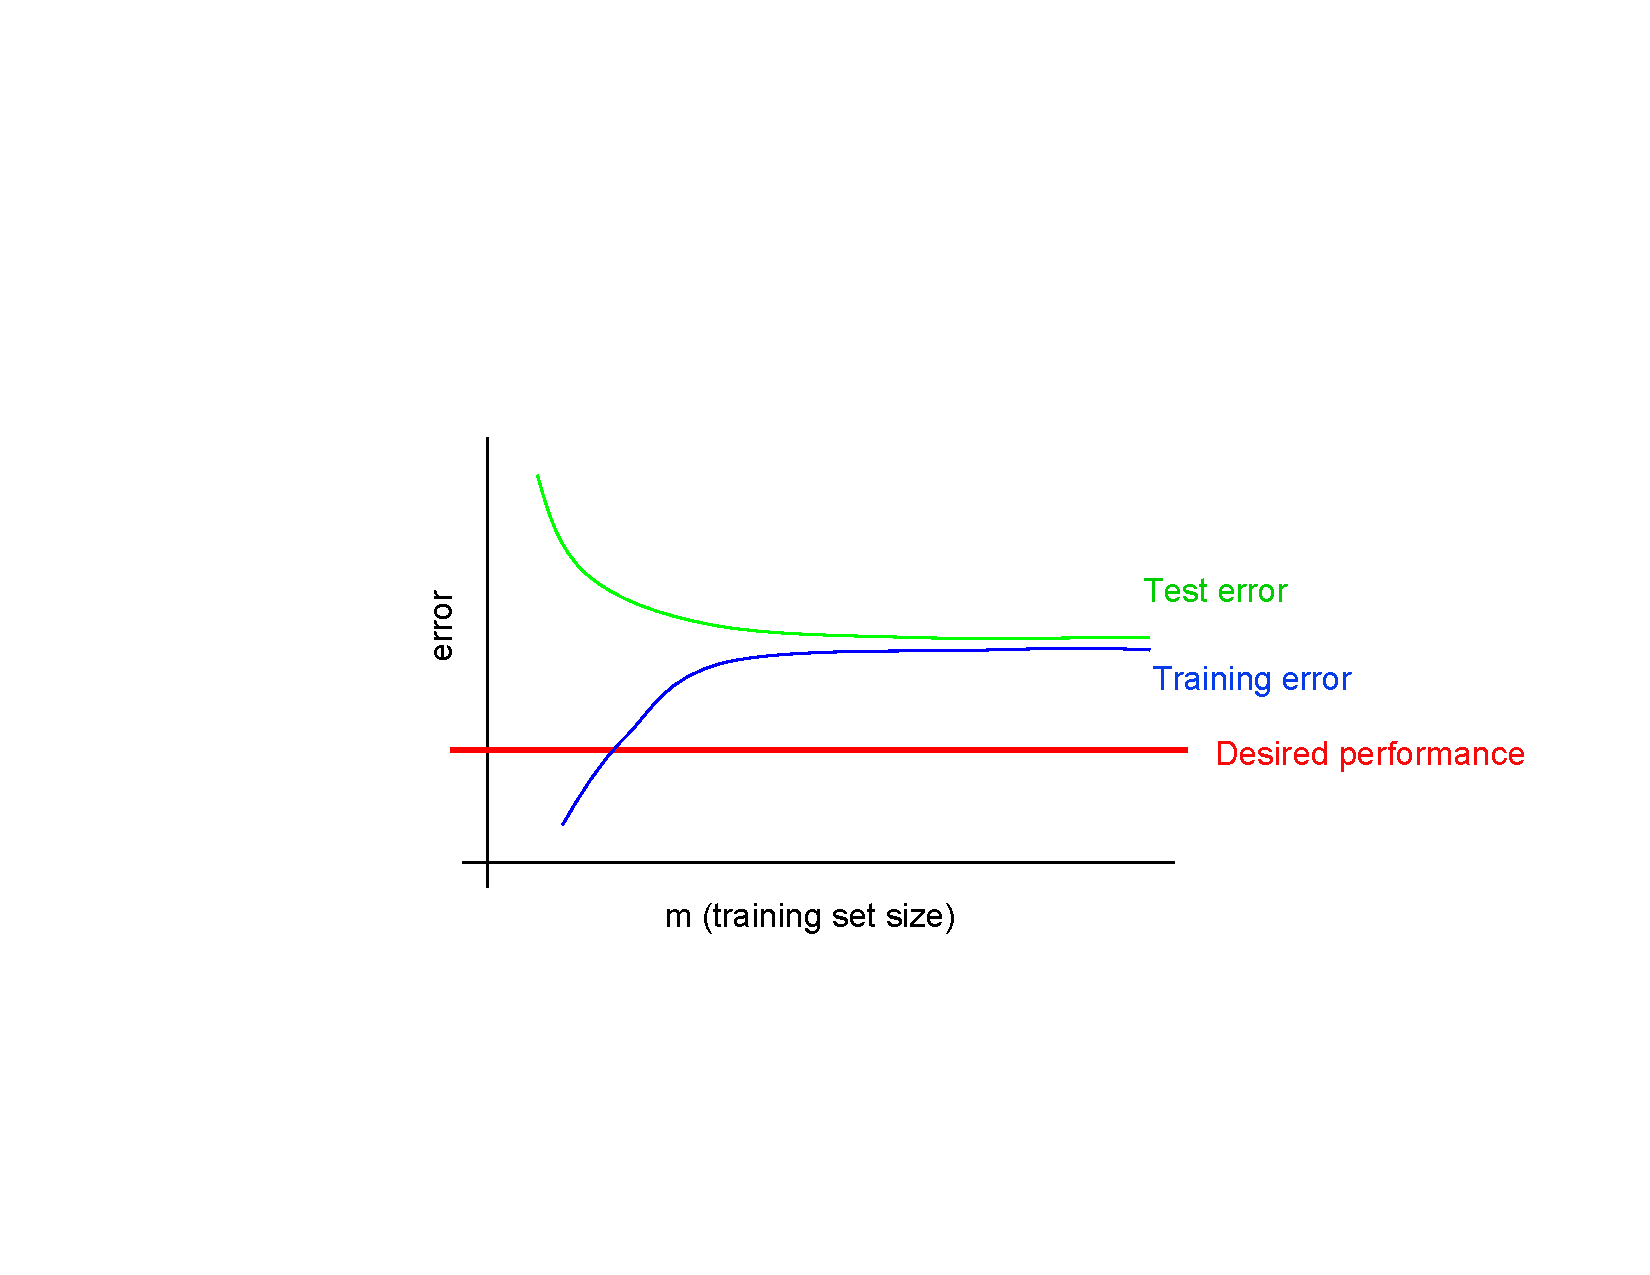
\includegraphics[width = 0.8\textwidth]{h_bia.pdf}
  \end{center}
  subraya las acciones que podrían mejorar al sistema de aprendizaje.

  \begin{itemize}
  \item Solicitarle a CFE información de otros 5 años anteriores.
  \item Disminuir el valor de $\lambda$ (parámetro de regularización).
  \item Aumentar el valor de $\lambda$ (parámetro de regularización).
  \item Utilizar solo la información histórica de los últimos 15 días y no de
    los 30 días anteriores.
  \item Utilizar una red neuronal en lugar de la regresión lineal.
  \item Agregar como atributos la raiz cuadrada de la demanda de energía
    eléctrica de los 30 días anteriores y la raiz cuadrada de los valores
    máximos y mínimos de temperatura de los 30 días anteriores.
  \item Agregar la humedad relativa de los 30 días anteriores.
  \end{itemize}

\item Sea la siguiente matriz de confusión, resuelta después de utilizar un
  método de aprendizaje para clasificar datos de un problema real:

  \begin{center}
    \begin{tabular}{cc}
      & $y$ \\
      $h_\theta(x)$ &
                      \begin{tabular}{c|cc}
                        & 0 & 1 \\
                        \hline
                        0 & 300 & 5 \\
                        1 & 10 & 30
                      \end{tabular}
    \end{tabular}
  \end{center}

  Responde a las siguientes preguntas:
  \begin{enumerate}
  \item ¿Cual es el error de clasificación? \line(1,0){80}
  \item ¿Cual es la precisión del clasificador? \line(1,0){80}
  \item ¿Cual es el \emph{recall} del clasificador? \line(1,0){80}
  \item ¿Cual es el $F_1$--score del clasificador? \line(1,0){80}
  \end{enumerate}


\end{enumerate}
\end{document}